\documentclass[10pt, twocolumn]{article}

\usepackage[a4paper, margin=0.5in]{geometry}
\usepackage{amsfonts}
\usepackage{amsthm}
\usepackage{amsmath}
\usepackage{parskip}
\usepackage{mathtools}
\usepackage{mathrsfs}
\usepackage{graphicx}
\usepackage{amssymb}
\usepackage{xtab}
\usepackage{physics}
\usepackage{algorithm}
\usepackage{algorithmic}
\usepackage{seqsplit}
\usepackage{enumitem}
\usepackage{tikz}
\usepackage{braket}
\usepackage{dirtytalk}
\usepackage{hyperref}
\usepackage{pgfplots}
\usetikzlibrary{quantikz}

\DeclareMathOperator{\lcm}{lcm}
\DeclarePairedDelimiter{\floor}{\lfloor}{\rfloor}
\DeclarePairedDelimiter{\ceil}{\lceil}{\rceil}
\DeclareMathOperator*{\argmax}{arg\,max}
\DeclareMathOperator*{\argmin}{arg\,min}

\newcommand*\diff{\mathop{}\!\mathrm{d}}

\newtheorem{theorem}{Theorem}[section]
\newtheorem{definition}[theorem]{Definition}
\newtheorem{proposition}[theorem]{Proposition}
\newtheorem{corollary}[theorem]{Corollary}
\newtheorem{lemma}[theorem]{Lemma}
\newtheorem{postulate}[theorem]{Postulate}
\newtheorem{problem}[theorem]{Problem}
\newtheorem*{claim}{Claim}


\usepackage[backend=biber, sorting=none]{biblatex}
\bibliography{bibliography}

\begin{document}

\title{QCE'24 Quantum Resource Estimation Educational Challenge Submission - Matrix Inversion by QSVT}
\author{Walden Killick}
\date{\textit{Cambridge Consultants, Cambridge, United Kingdom}}

\maketitle

\begin{abstract}
	We investigate the physical resources required to solve systems of linear equations using the quantum singular value transform algorithm. We find that empirically, both the qubit counts and runtimes scale favorably (polylogarithmically) with the input size. By extrapolating the data, we predict that a $10^{10}$-dimensional matrix may be inverted using under 2 million qubits in about one hour. We furthermore identify bottlenecks in the scaling and highlight opportunities for further optimization.
\end{abstract}

\section{Introduction}

Since the breakthrough 2009 algorithm of Harrow, Hassidim, and Lloyd (HHL algorithm), it has been well-known that for sparse, well-conditioned matrices, quantum computers are capable of solving the system of linear equations (SLE) problem exponentially faster than the best possible classical algorithms \cite{harrow2009quantum}. Due to the complexities of practical implementation, the performance analyses of quantum algorithms for solving SLEs have been primarily restricted to the asymptotic regime. In this project, we aim to answer the question of what physical quantum resources are required to solve SLEs of sizes at which the problem becomes classically intractable. Specifically, we consider the use of the quantum singular value transformation (QSVT) which achieves the best asymptotic complexity of all known quantum SLE algorithms \cite{gilyen2019quantum, martyn2021grand}.

All code used to generate the results in this report can  be found at \href{https://github.com/Walden-Killick/QCE24-QRE-Challenge}{https://github.com/Walden-Killick/QCE24-QRE-Challenge}.

\section{Preliminary}

\subsection{Problem definition}

Given a quantum state $\ket{b}$ and an efficient classical description of a sparse matrix $A$, the quantum system of linear equations (QSLE) problem is the problem of preparing the state $\ket{x} = A^{-1} \ket{b}$. Broadly speaking, the primary challenges in any QSLE algorithm are (1) accessing $A$ in a quantum circuit, and (2) performing (approximately) the transformation $A \mapsto A^{-1}$. The HHL algorithm \cite{harrow2009quantum} achieves these goals using a sparse Hamiltonian simulation subroutine \cite{berry2007efficient} and quantum phase estimation \cite{kitaev1995quantum}, respectively. By contrast, QSVT utilizes the fundamentally different techniques of block encoding \cite{gilyen2019quantum} and quantum signal processing \cite{low2017optimal} and achieves an exponentially improved dependence on the target precision as well as a lesser improvement with respect to the condition number. We briefly review these techniques in the following subsection.

\subsection{Matrix inversion by QSVT}

To access $A$ in a quantum circuit, QSVT relies on quantum oracles which efficiently encode both the non-zero structure and non-zero elements of $A$. These are defined rigorously as follows.

\begin{definition}[Sparse access oracles \cite{camps2203explicit}]
	\label{def::sparse_access_oracles}
	Let $A$ be an $N \times N$ $s$-sparse\footnote{A matrix is \textit{$s$-sparse} if it has at most $s$ non-zero entries per column.} matrix. Let $c(j,l)$ be a function which returns the row index of the $l$-th non-zero matrix element in the $j$-th column of $A$. The sparse access oracles $O_c$ and $O_A$ for $A$ are the unitary operators defined as
	\[
		O_c \ket{l}\ket{j} = \ket{l}\ket{c(j, l)}
	\]
	and
	\[
		O_A \ket{0}\ket{l}\ket{j} = \left( A_{c(j, l), j} \ket{0} + \sqrt{1 - \abs{A_{c(j, l), j}}^2 } \ket{1} \right) \ket{l} \ket{j}.
	\]
\end{definition}

We should note that in this formalism, $O_A$ also implicitly encodes the non-zero structure of $A$ by calling $c(j, l)$; however, for certain sufficiently well-structured matrices such as those considered in this project, this is not prohibitive.

The following informal theorem states that one can construct a unitary matrix which directly contains (a down-scaled version of) $A$ as a submatrix (block).

\begin{theorem}[Block-encoding sparse matrices \cite{gilyen2019quantum, camps2203explicit}]
	\label{thm::block_encoding_sparse_matrices}
	Let $A, O_c, O_A$ be as in Definition \ref{def::sparse_access_oracles}. Using one call to each of $O_c$ and $O_A$, we can construct a larger unitary matrix $U_A$ for which the upper left $N \times N$ block is equal to $A/s$.
\end{theorem}

The final ingredient in matrix inversion by QSVT is then to transform the singular values of $A/s$ as $x \mapsto 1/x$. QSVT cannot perform this transformation exactly, but can perform almost-arbitrary polynomial transformations \cite{sunderhauf2023generalized} and thus approximate $1/x$ to arbitrary precision.

\begin{theorem}[Matrix inversion by QSVT \cite{gilyen2019quantum}]
	\label{thm::matrix_inversion_by_qsvt}
	Let $A$ be a sparse matrix with condition number $\kappa$ and let $U_A$ block-encode $A$ as in Theorem \ref{thm::block_encoding_sparse_matrices}. Using $O(\kappa \log(\kappa / \varepsilon))$ calls to $U_A$ and $U_A^\dag$, we can construct a unitary which block-encodes $A^{-1}$ to within accuracy $\varepsilon$.
\end{theorem}

We refer the reader to \cite{martyn2021grand} for a pedagogical introduction to block encodings and QSVT.

\subsection{Banded circulant matrices}

To construct polynomial-size oracles $O_c$ and $O_A$, $A$ must be well-structured in some way. For this project, we consider \textit{banded circulant} matrices primarily as they are amongst the simplest classes of matrices which can be block-encoded efficiently whilst still exhibiting nontrivial solutions.

\begin{definition}[Circulant matrix]
	A circulant matrix is a matrix in which each row is equal to the previous row but with each element shifted one place to the right.
\end{definition}

\begin{definition}[Banded circulant matrix]
	A circulant matrix is banded if only the first three entries of the second row are non-zero.
\end{definition}

The following is an example of a banded circulant matrix with diagonal entries $\alpha$, sub-diagonal entries $\beta$, and super-diagonal entries $\gamma$:
\[
	\begin{bmatrix}
		\alpha & \gamma & 0 & \cdots & \beta \\
		\beta & \alpha & \gamma & \cdots & 0 \\
		0 & \beta & \alpha & \cdots & 0 \\
		\vdots & \vdots & \vdots & \ddots & \vdots \\
		\gamma & 0 & 0 & \cdots & \alpha
	\end{bmatrix}.
\]
Physically, a banded circulant matrix corresponds to the adjacency matrix of a cycle graph.

Reference \cite{camps2203explicit} shows how to construct polynomial-size sparse-access oracles for this class of matrices, for which we show a high-level sketch in Figure \ref{fig::block_encoding_circuit}. In particular, the authors show how to construct $O_A$ in $O(1)$ time and $O_c$ in $O(\text{poly}\log(N))$ time. Combining this with Theorems \ref{thm::block_encoding_sparse_matrices} and \ref{thm::matrix_inversion_by_qsvt}, we can see that using the aforementioned construction, we can perform matrix inversion by QSVT in time $O(\kappa \, \text{poly}\log(N) \log(\kappa / \varepsilon))$, retaining the exponential quantum speedup with respect to the matrix size. This furthermore outperforms the HHL algorithm with respect to both precision and the condition number, which has a complexity of $O(\kappa^2 \log(N) / \varepsilon)$ \cite{harrow2009quantum}.

\begin{figure}
	\centering
	\begin{quantikz}[column sep = 2pt]
		& \qw & \qw & \gate{R_Y(\theta_0)}\gategroup[3, steps = 3, style = {dashed, rounded corners, inner xsep = 2pt, inner ysep = 2pt} ]{$O_A$} & \gate{R_Y(\theta_1)} & \gate{R_Y(\theta_2)} & \qw & \qw & \qw & \qw & \qw & \qw \\
		& \gate{H} & \hphantomgate{} & \octrl{-1} & \octrl{-1} & \ctrl{-1} & \qw & \qw\gategroup[3, steps = 2, style = {dashed, rounded corners, inner xsep = 2pt, inner ysep = 2pt}, label style = {label position = below, anchor = north, yshift = -6pt}]{$O_c$} & \ctrl{2} & \hphantomgate{} & \gate{H} & \qw \\
		& \gate{H} & \qw & \octrl{-1} & \ctrl{-1} & \octrl{-1} & \qw & \ctrl{1} & \qw & \qw & \gate{H} & \qw \\
		& \qwbundle{n = \ceil{\log{N}}} & \qw & \qw & \qw & \qw & \hphantomgate{} & \gate{L} & \gate{R} & \qw & \qw & \qw
	\end{quantikz}
	\caption{Quantum circuit for block-encoding an $N \times N$ banded circulant matrix, adapted from \cite{camps2203explicit}. For $n = \ceil{\log{N}}$ qubits, the $L$ and $R$ gates each consist of $n$ multi-controlled \textsc{NOT} gates with successively decreasing numbers of controls (see Figure \ref{fig::shift_gate_circuits}).}
	\label{fig::block_encoding_circuit}
\end{figure}

\begin{figure}
	\centering
	\begin{quantikz}
		\lstick[3]{$n$} & & \targ{} & \qw & \qw & \qw \\
		& & \ctrl{-1} & \targ{} & \qw & \qw \\
		& & \ctrl{-1} & \ctrl{-1} & \gate{X} & \qw
	\end{quantikz}
	\quad
	\begin{quantikz}
		\qw & \targ{} & \qw & \qw & \qw \\
		\qw & \octrl{-1} & \targ{} & \qw & \qw \\
		\qw & \octrl{-1} & \octrl{-1} & \gate{X} & \qw
	\end{quantikz}
	\caption{Quantum circuits for the $L$ and $R$ gates respectively, with $n=3$ qubits.}
	\label{fig::shift_gate_circuits}
\end{figure}

\section{Results}

The resource estimates were generated by exporting Qiskit QSVT circuits to OpenQASM 2 files and subsequently loading them into the Microsoft Azure Quantum Resource Estimator via the web portal. We are primarily concerned with observing how the resource estimates scale with the input size $N$, and thus arbitrarily assume condition number $\kappa=3$ and target accuracy $\varepsilon=0.1$ for all circuits. The QASM circuits and the scripts used to generate them can be found in the folder \href{https://github.com/Walden-Killick/QCE24-QRE-Challenge/tree/main/qasm_circuits}{\textsc{qasm\_circuits}}.

\subsection{Qubit counts}

Figure \ref{fig::qre_qubits} shows how the logical and physical resource estimates scale with the input size. Whilst the logical qubit estimates conform very naturally with the expected logarithmic growth, the physical estimates scale much more erratically. We attribute this to the `lucky' cancellation of non-Clifford gates when transpiling the $L$ and $R$ gates (see Figure \ref{fig::shift_gate_circuits}), since the anomalously low results are caused by smaller $T$ factory count estimates. In the interest of extrapolating to worst-case resource estimates, we mark as outliers the instances which outperform an instance of smaller size (indicated with hollow markers in Figure \ref{fig::qre_qubits}). Promisingly, despite the somewhat irregular results, the physical resource estimates nonetheless likewise conform to a logarithmic growth with $N$.

The logarithmic best-fit functions, computed using NumPy's polyfit, are roughly:
\begin{align*}
	y_\text{logical} &\approx 3.61 \log{N} + 15.2, \\
	y_\text{physical} &\approx 67800 \log{N} + 219000,
\end{align*}
where $\log$ denotes the natural logarithm.

Although highly impractical for small problem sizes due to the large constant factors, the data would seem to empirically imply that a realistically achievable number of physical qubits will be able to tackle problems of classically intractable sizes. For example, if the extrapolation of the physical qubit requirements remains accurate for large inputs, a $10^{10}$-dimensional banded circulant matrix could be inverted using under 2 million physical qubits.

\begin{figure}
	\centering
	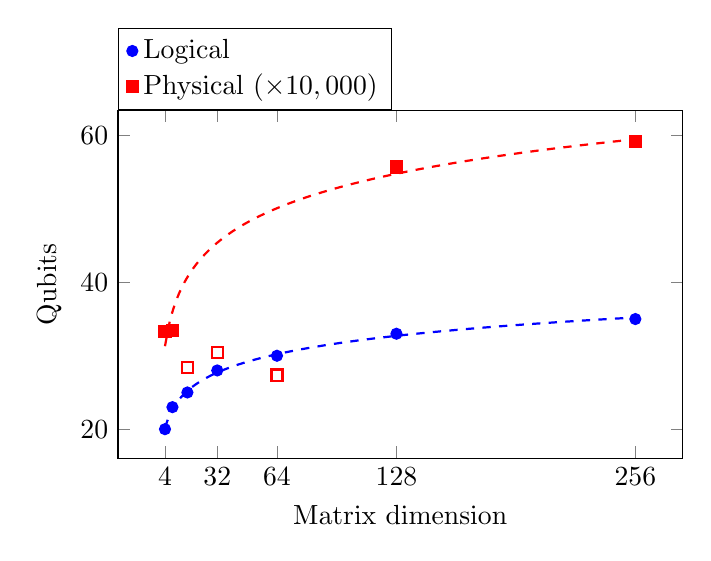
\begin{tikzpicture}
		\begin{axis}[xlabel=Matrix dimension, ylabel=Qubits, xtick={4, 32, 64, 128, 256}, width=8.75cm, height=6cm, legend style={at={(0,1)}, legend cell align={left}, anchor = south west}]
			\addplot[mark=*, only marks, color=blue] coordinates{(4,20)(8,23)(16,25)(32,28)(64,30)(128,33)(256,35)};
			\addlegendentry{Logical};
			\addplot[mark=square*, only marks, color=red, thick] coordinates{(4,33.3)(8,33.435)(128,55.695)(256,59.171)};
			\addplot[mark=square, only marks, color=red, thick] coordinates{(16,28.445)(32,30.418)(64,27.366)};
			\addlegendentry{Physical ($\times 10,000$)};
			\addplot[domain = 4:256, samples=100, smooth, thick, dashed, color=blue] {3.6067376022224074*ln(x)+15.214285714285719};
			\addplot[domain = 4:256, samples=100, smooth, thick, dashed, color=red] {(67769.48978034298*ln(x)+219131.34615384619)/10000};
		\end{axis}
	\end{tikzpicture}
	\caption{Resource estimates for the logical and physical qubit requirements for matrix inversion by QSVT.}
	\label{fig::qre_qubits}
\end{figure}

\subsection{Runtimes}

Figure \ref{fig::qre_runtime} shows how the runtime estimates scale with the input size. In this case, the asymptotic growth of the runtime at first glance appears linear as opposed to the desired polylogarithmic growth. Although more data points could theoretically be used to verify the behavior, an additional challenge faced here is that the resource estimator reaches its maximum timeout of 20 minutes for matrices of size greater than 256.

\begin{figure}
	\centering
	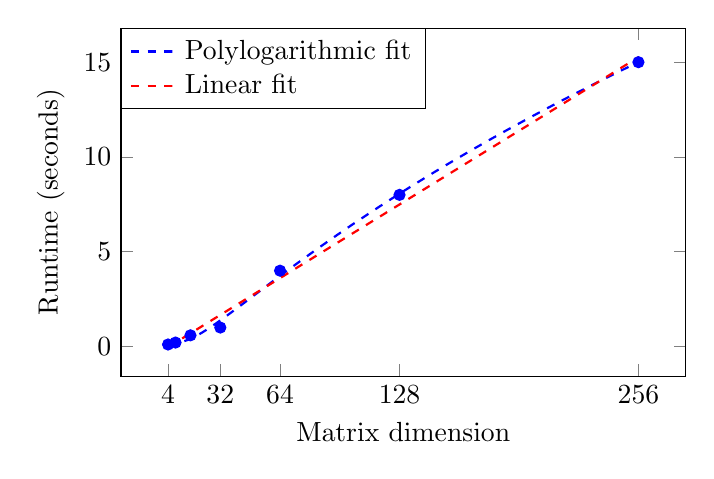
\begin{tikzpicture}
		\begin{axis}[xlabel=Matrix dimension, ylabel=Runtime (seconds), xtick={4, 32, 64, 128, 256}, width=8.75cm, height=6cm, legend style={at={(0,1)}, legend cell align={left}, anchor = north west}]
			\addplot[domain = 4:256, samples=100, smooth, thick, dashed, color=blue] {0.30803527840088796*ln(x)^3 - 1.771517817276902*ln(x)^2 + 3.424306187979826*ln(x) - 2.033572179167546};
			\addlegendentry{Polylogarithmic fit};
			\addplot[domain = 4:256, samples=100, smooth, thick, dashed, color=red] {0.06069840030772014*x - 0.27568390804597964};
			\addlegendentry{Linear fit};
			\addplot[mark=*, only marks, color=blue] coordinates{(4,0.106)(8,0.209)(16,0.590)(32,1)(64,4)(128,8)(256,15)};
		\end{axis}
	\end{tikzpicture}
	\caption{Resource estimates for the running time of matrix inversion by QSVT.}
	\label{fig::qre_runtime}
\end{figure}

To circumvent this issue, we first note that the only circuit elements that change size between instances are the $L$ and $R$ gates (see Figure \ref{fig::block_encoding_circuit}) which ultimately consist of several multi-controlled \textsc{NOT} gates (see Figure \ref{fig::shift_gate_circuits}). In the exploratory notebook \href{https://github.com/Walden-Killick/QCE24-QRE-Challenge/blob/main/notebooks/exploration/qiskit_transpilation.ipynb}{\textsc{qiskit\_transpilation.ipynb}}, we have empirically found the runtime of Qiskit's transpilation of multi-controlled gates to scale as $O(n^2)$, implying a `naive' implementation such as the construction found in \cite{barenco1995elementary}. With the number of such gates present in the block-encoding circuit, we should then expect to see a runtime scaling of $O(n^3) = O(\log^3{N})$. Fitting the data to a degree-3 polylogarithmic function using SciPy's curve\_fit yields
\[
	y_\text{runtime} = 0.308 \log^3{N} - 1.77 \log^2{N} + 3.42 \log{N} - 2.03
\]
which indeed conforms to the dataset with a smaller average error than the linear fit. To further justify fitting to this function, in the notebook \href{https://github.com/Walden-Killick/QCE24-QRE-Challenge/blob/main/notebooks/results/block_encoding_runtime.ipynb}{\textsc{block\_encoding\_runtime.ipynb}} we have evaluated the runtime of the block-encoding circuit only and observed clear polylogarithmic scaling, which implies that the same scaling holds for the full QSVT circuit.

If the extrapolation to higher dimensional matrices remains accurate, with this implementation a $10^{10}$-dimensional banded circulant matrix could be inverted on a quantum computer in about one hour.

\section{Conclusion and discussion}

Whilst of significant practical relevance, quantum algorithms for solving SLEs are still predominantly presented in a complexity-theoretic and oracular, and rarely a practical, setting. In this project, we have built explicit quantum circuits for solving SLEs by QSVT for a specific class of sparse matrices, and evaluated the end-to-end physical resource requirements using Microsoft's Azure Quantum Resource Estimator.

Our findings show that both the logical and physical qubit count estimates adhere to the expected logarithmic growth, and that a realistically achievable number of physical qubits may suffice to demonstrate quantum advantage for matrix inversion.

The resource estimates for runtime seem to display a lesser degree of certainty in their asymptotic growth with matrix size, but we can deduce both theoretically and empirically that we should expect to see a growth which scales as $O(\log^3{N})$. Fitting the data as such, if the behavior remains consistent when extrapolated to large matrix sizes, we should likewise expect a reasonable amount of time to suffice to invert matrices of classically challenging sizes.

We furthermore highlight room for optimization in these estimates. When scaling to large matrices, we are bottlenecked by the many multi-controlled \textsc{NOT} gates present in $O_c$ (see Figure \ref{fig::shift_gate_circuits}). The software tools we have used appear to transpile such gates into circuits of depth $O(n^2)$, resulting in an overall complexity for $O_c$ of $O(\log^3{N})$. The best way to transpile multi-controlled gates is an area of active research, with recent theoretical results achieving depths as low as $O(\log^3{n})$ \cite{claudon2024polylogarithmic}. With the $n \sim \log{N}$ gates present in $L$ and $R$, this would imply an overall runtime which scales with input size as $O(n \log^3{n}) = O(\log{N} \log^3{\log{N}} )$. If and by how much these results reduce resource requirements in practice remains an open question and a potential direction for future work.

\printbibliography

\end{document}